\documentclass[a4paper]{article}
\usepackage[affil-it]{authblk}
\usepackage{amsthm,amsmath,amssymb}
\usepackage{geometry}
\usepackage{graphicx}
\usepackage{subcaption}

\geometry{margin=1.5cm, vmargin={0pt,1cm}}
\setlength{\topmargin}{-1cm}
\setlength{\paperheight}{29.7cm}
\setlength{\textheight}{25.3cm}
\newcommand{\QED}{\hfill\ensuremath{\square}}

\begin{document}

% =================================================
\title{Numerical Analysis Programming Report 2}

\author{Chen Wanqi 3220102895
  \thanks{Electronic address: \texttt{3220102895@zju.edu.cn}}}
\affil{Information and Computer Science 2201, Zhejiang University}

\date{\today}

\maketitle

%=================================================

\section*{Problem A}
The task is to write a program for Newton's interpolation polynomial, the specific implementation can be seen in ./src/interpolation.h and ./src/interpolation.cpp, and the design document can be found in ./DesignDoc.md.

\section*{Problem B}

Given the function
\[
    f(x) = \frac{1}{1+x^2},
\]
and the rule for selecting interpolation points
\[
    x_i = -5 + 10\frac{i}{n}, \quad i = 0,1,2,...,n; \quad (n = 2,4,6,8)
\]
test the program of Newton's interpolation polynomial from Problem A.

1. First, define the target function \( f(x) = \frac{1}{1 + x^2} \).

2. For each \( n \), select the corresponding interpolation points according to the formula \( x_i = -5 + 10\frac{i}{n}, \, i = 0,1,2,...,n \), store them in the array x\_vals, and calculate the corresponding function values, stored in the array f\_vals.

3. Call the initialization function of the NewtonInterpolator class to construct an instance, call the interpolate function to obtain the interpolation polynomial, and use the print function of the Polynomial class to output the polynomial expression.

4. To plot the image of the interpolation polynomial and compare it with the original function, use the evaluate function to calculate the values of the interpolation polynomial within the domain, store them in the file ./data/ProblemB.dat, and then use ./plot/plot\_ProblemB.py to draw the image.

The plotted image is as follows:
\begin{figure}[h]
    \centering
    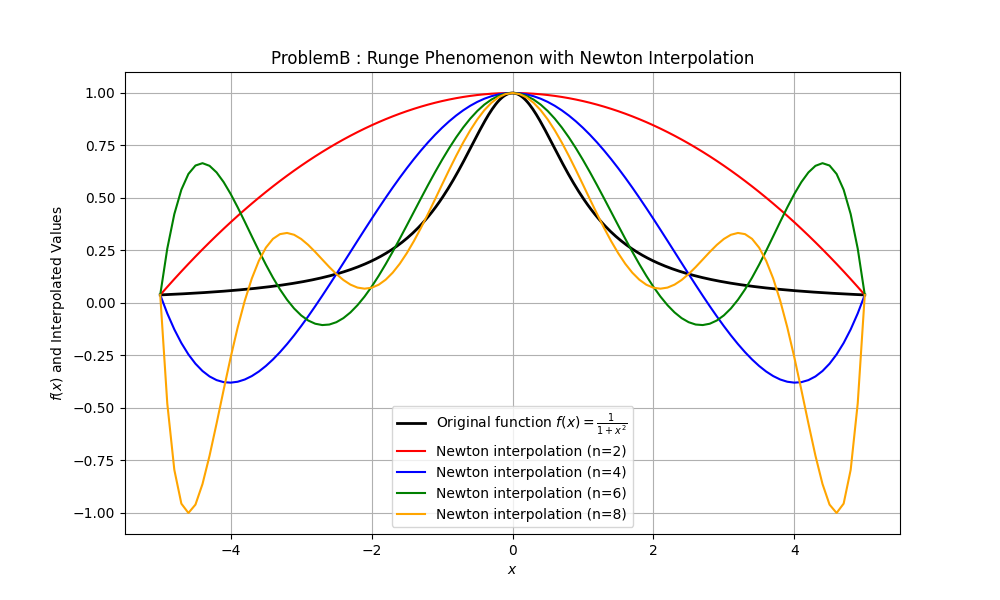
\includegraphics[width=0.75\linewidth]{Pictures/ProblemB_figure.png}
    \label{fig:enter-label}
\end{figure}

It can be seen that the larger the \( n \), the better the fitting effect of the interpolation polynomial with the original function.

\newpage
\section*{Problem C}

In this problem, we performed Chebyshev interpolation on the given function 
\[
f(x) = \frac{1}{1 + 25x^2}
\]
to improve the stability and fitting accuracy of the interpolation. We chose the zeros of the Chebyshev polynomial as the interpolation nodes, avoiding the Runge phenomenon. The selected interpolation points satisfy
\[
x_i = \cos \left( \frac{(2i + 1) \pi}{2n} \right), \quad i = 0, 1, 2, \ldots, n - 1,
\]
where \( n = 5, 10, 15, 20 \).

1. First, define the target function \( f(x) = \frac{1}{1 + 25 x^2} \).

2. Use the formula \( x_i = \cos \left( \frac{(2i + 1) \pi}{2n} \right) \) to generate Chebyshev interpolation points, store the results in the x\_vals array. Calculate the function values corresponding to each interpolation point and store them in the f\_vals array.

3. Construct an instance of NewtonInterpolator for each \( n \), and generate the corresponding interpolation polynomial Polynomial by calling the interpolate method.

4. Use the evaluate function to calculate the values of the interpolation polynomial on the interval \([-1, 1]\), and store the results in the file ./data/ProblemC.txt for subsequent use with ./plot/plot\_ProblemC.py to draw the image.

The figure below shows the fitting effect of the interpolation polynomial and the original function:
\begin{figure}[h]
    \centering
    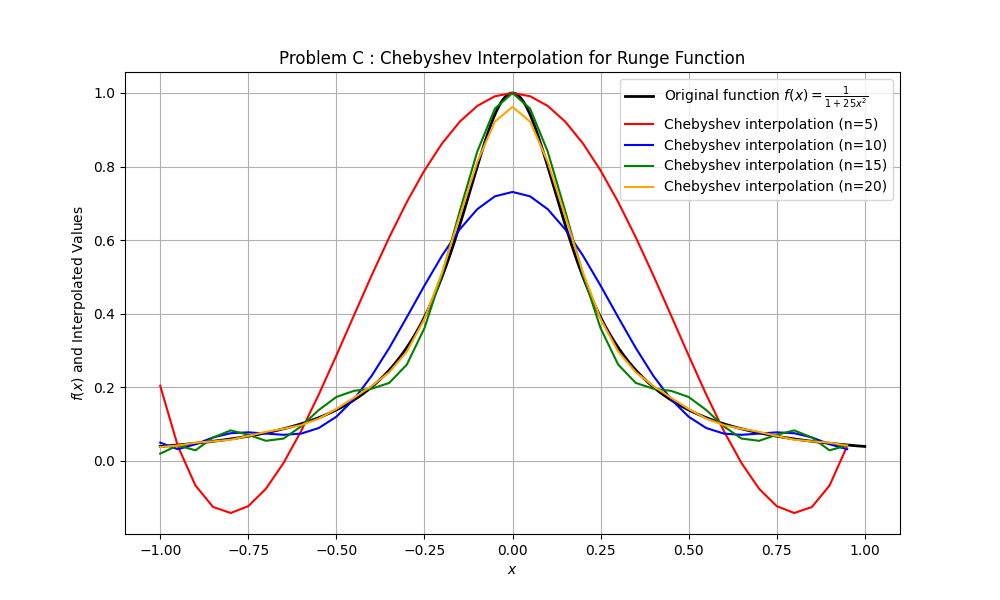
\includegraphics[width=0.75\linewidth]{Pictures/ProblemC_figure.png}
    \label{fig:enter-label}
\end{figure}

By observing the image, it can be found that as \( n \) increases, the interpolation polynomial gradually gets closer to the original function, especially the fitting effect near the interval endpoints is significantly improved. This shows that Chebyshev interpolation performs well in reducing edge errors and enhancing overall fitting effects.

\newpage
\section*{Problem D}

The problem requires predicting the position and velocity of a car at \( t = 10 \) seconds based on the observation data shown in the table below using Hermite interpolation polynomial:

\[
\begin{array}{|c|c|c|}
\hline
\text{Time (s)} & \text{Displacement (ft)} & \text{Velocity (ft/s)} \\
\hline
0 & 0 & 75 \\
3 & 225 & 77 \\
5 & 383 & 80 \\
8 & 623 & 74 \\
13 & 993 & 72 \\
\hline
\end{array}
\]

1. First, input the observation data required for Hermite interpolation, stored in the time, displacement, velocity three arrays.

2. Call the initialization function of the HermiteInterpolator class to construct an instance, and finally call the interpolate function to obtain the Hermite interpolation polynomial (the relationship between distance and time), use the derivative function of the Polynomial class to calculate the derivative to get the relationship between velocity and time.

3. Output the velocity and displacement polynomials to the ./data/ProblemD.txt file for use with ./plot/plot\_ProblemD.py to draw the image.

4. Call the evaluate function to calculate the position and velocity of the Hermite interpolation polynomial at \( t = 10 \) seconds, and output the results.

(a) According to the output results at \( t = 10 \, s \), Displacement= 742.503 feet, Velocity= 48.3817 feet/second.

(b) According to the plotted image, it can be seen that the car was speeding during this period.

The figure below shows the fitting effect of the Hermite interpolation polynomial and the original data:
\begin{figure}[h]
    \centering
    \begin{subfigure}[b]{0.45\textwidth}
        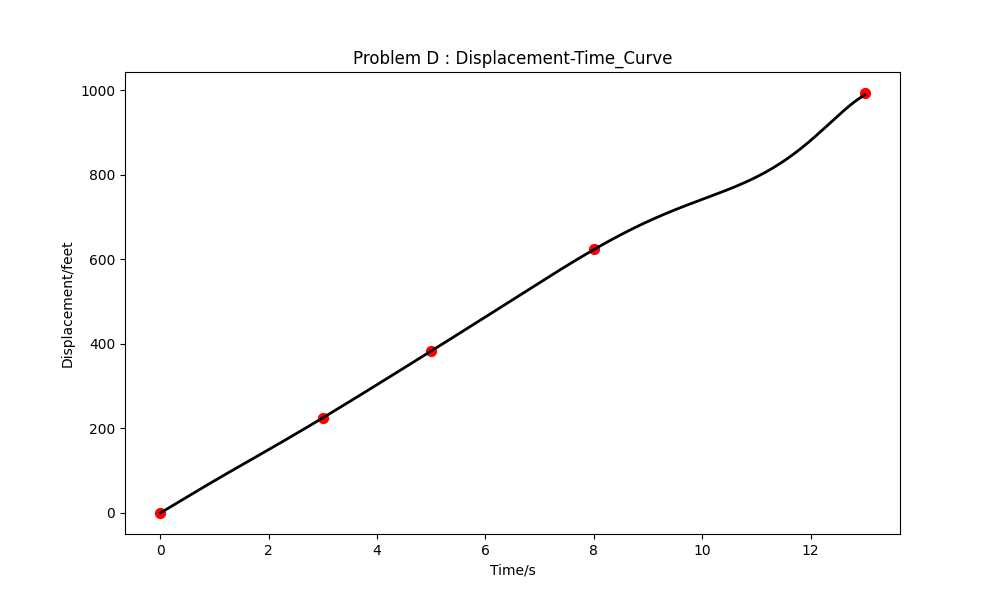
\includegraphics[width=\textwidth]{Pictures/ProblemD_figure_Displacement-Time_Curve.png}
    \end{subfigure}
    \hfill
    \begin{subfigure}[b]{0.45\textwidth}
        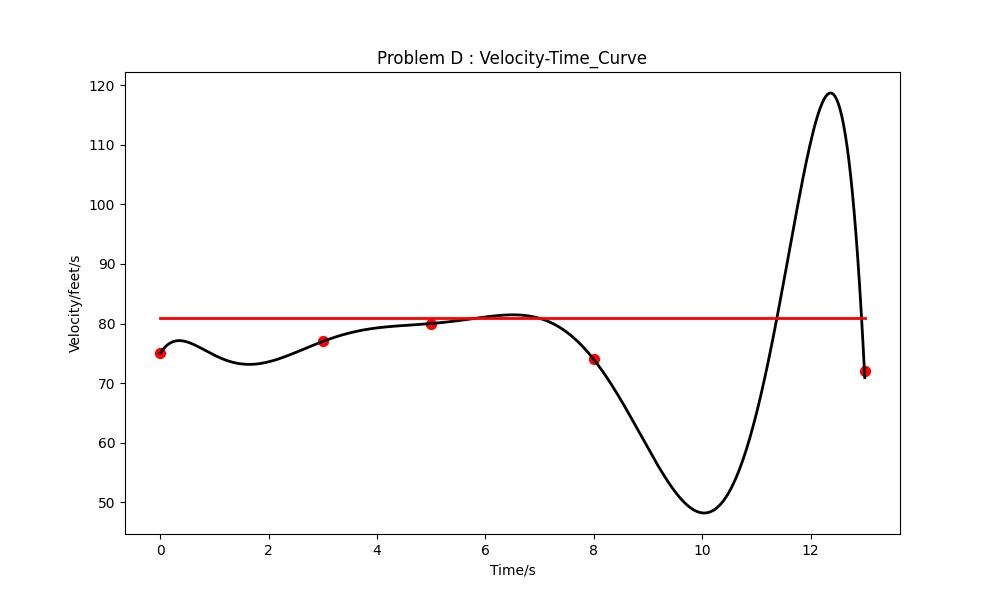
\includegraphics[width=\textwidth]{Pictures/ProblemD_figure_Velocity-Time_Curve.png}
    \end{subfigure}

\end{figure}

\newpage
\section*{Problem E}

The problem requires predicting the change of weight over time for two samples based on the observation data shown in the table below using Newton's interpolation polynomial:

\[
\begin{array}{|c|c|c|}
\hline
\text{Day} & \text{Sample 1 Weight (g)} & \text{Sample 2 Weight (g)} \\
\hline
0 & 6.67 & 6.67 \\
6 & 17.3 & 16.1 \\
10 & 42.7 & 18.9 \\
13 & 37.3 & 15.0 \\
17 & 30.1 & 10.6 \\
20 & 29.3 & 9.44 \\
28 & 28.7 & 8.89 \\
\hline
\end{array}
\]

1. First, input the observation data required for Newton's interpolation, stored in the days, sp1\_weights, sp2\_weights three arrays.

2. Perform Newton's interpolation to obtain the polynomials for the change in weight over time for the two samples, and output them to the file ./data/ProblemE.txt, use ./plot/plot\_ProblemE.py to draw the image.

3. Call the evaluate function to calculate the weight of the two samples at \( t = 43 \) days, and output the results.

(a) From the output results, it can be seen:
\begin{verbatim}
Sample 1 Weight-Time Polynomial:
0.00x^6 -0.00x^5 +0.13x^4 -2.12x^3 +16.29x^2 -43.01x^1 +6.67x^0
Sample 2 Weight-Time Polynomial:
0.00x^6 -0.00x^5 +0.03x^4 -0.42x^3 +2.98x^2 -5.85x^1 +6.67x^0
\end{verbatim}


(b) From the output results, it can be seen:
\begin{verbatim}
Predicted Weight of Sample 1 at \( t = 43.00 \): 14640.26 grams
Predicted Weight of Sample 2 at \( t = 43.00 \): 2981.48 grams
\end{verbatim}


The figure below shows the change in weight over time for the two samples:

\begin{figure}[h]
    \centering
    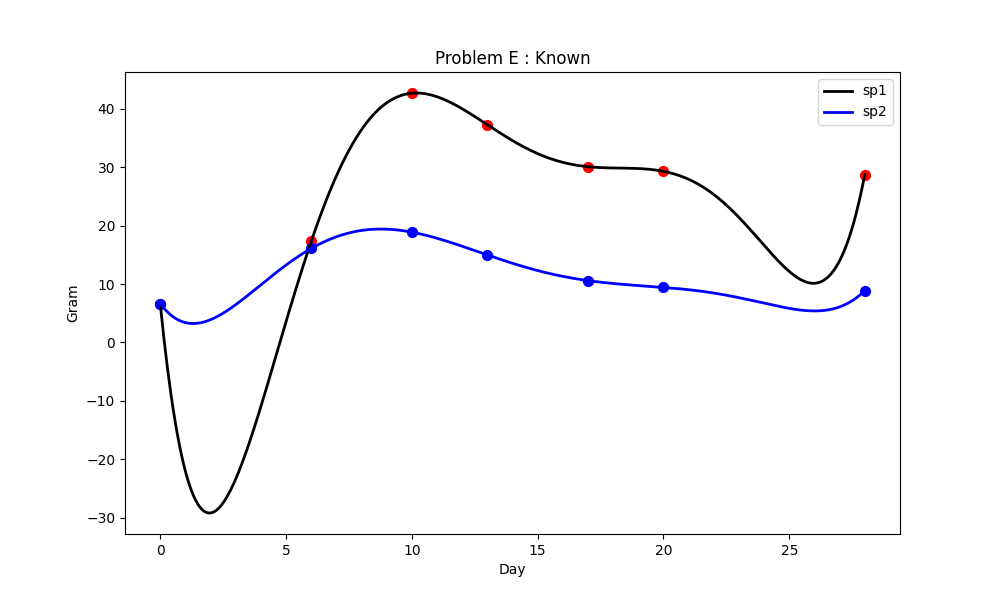
\includegraphics[width=0.75\linewidth]{Pictures/ProblemE_figure_Known.png}
    \label{fig:enter-label}
\end{figure}

It can be seen that the fitting effect is good.

\newpage
The figure below is the prediction of the change in weight over time for the two samples to 43 days:

\begin{figure}[h]
    \centering
    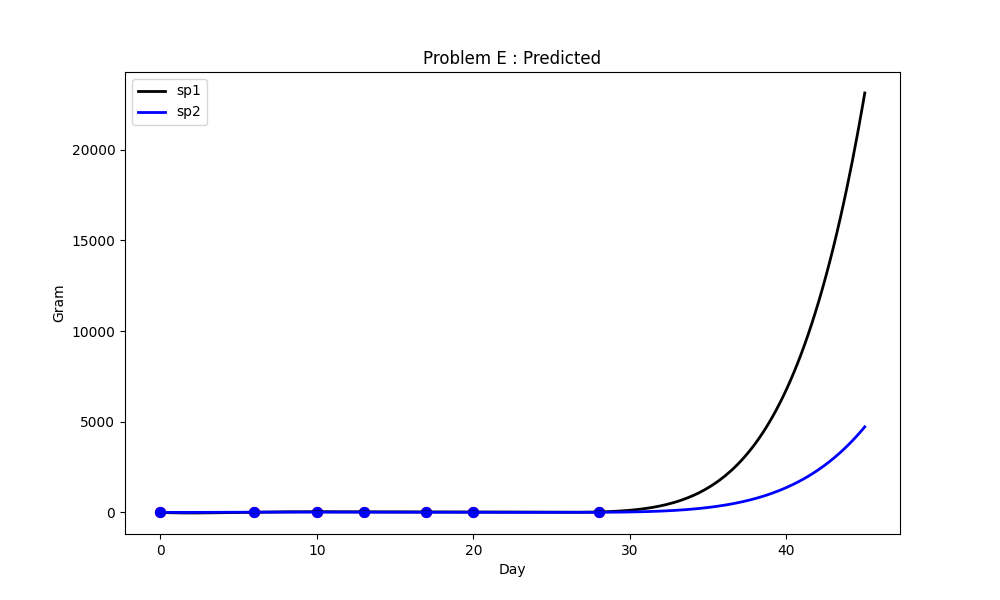
\includegraphics[width=0.75\linewidth]{Pictures/ProblemE_figure_Predicted.png}
    \label{fig:enter-label}
\end{figure}

It can be seen that after more than 30 days, the weight increase rate of the two samples has an abnormal increase, indicating that Newton's interpolation has poor predictive effect outside the given interpolation point range.


\section*{Problem F}

This problem gives the expression of the heart-shaped curve
\[
    x^2 + \left(\frac{3}{2}y - \sqrt{|x|}\right)^2 = 3
\]
and requires fitting the heart-shaped curve with Bezier curves.

1. First, define the heart-shaped curve function heart\_function, and the tangent vector function heart\_tangent.

2. Set the value of \( m \), for each \( m \), within the domain \((-\sqrt{3},\sqrt{3})\), call find\_points to uniformly select \( m+1 \) points, uniform point selection is beneficial to the fitting effect of all points of the fitted Bezier curve.

3. Use the convert\_to\_control\_points function to convert \( m+1 \) points into \( m \) groups of Bezier curve control points, each group contains 4 points.

4. Construct the Bezier curve in turn with the control points of the \( m \) groups, call the fileOut function to output the results. Use ./plot/plot\_ProblemF.py to draw the image.

It is noted here that if the selected points are not sorted in a clockwise or counterclockwise order, the drawn image will appear as shown in the following figure:
\begin{figure}[h]
    \centering
    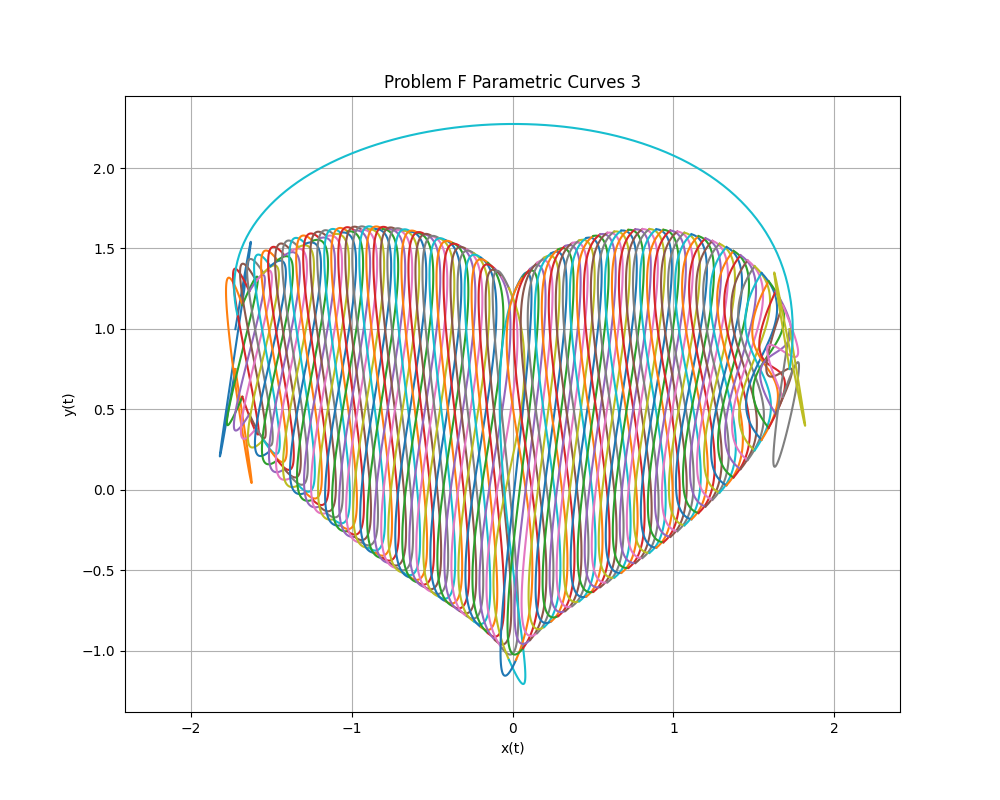
\includegraphics[width=0.45\linewidth]{Pictures/ProblemF_withoutsort.png}
    \label{fig:enter-label}
\end{figure}

\newpage
Therefore, we calculated the polar angle of the selected points in the find\_points function and sorted the points in ascending order of the polar angle, resulting in the following fitting effect: fitting effects when \( m = 10, 40 \), and 160.

\begin{figure}[h]
    \centering
    \begin{subfigure}[b]{0.45\textwidth}
        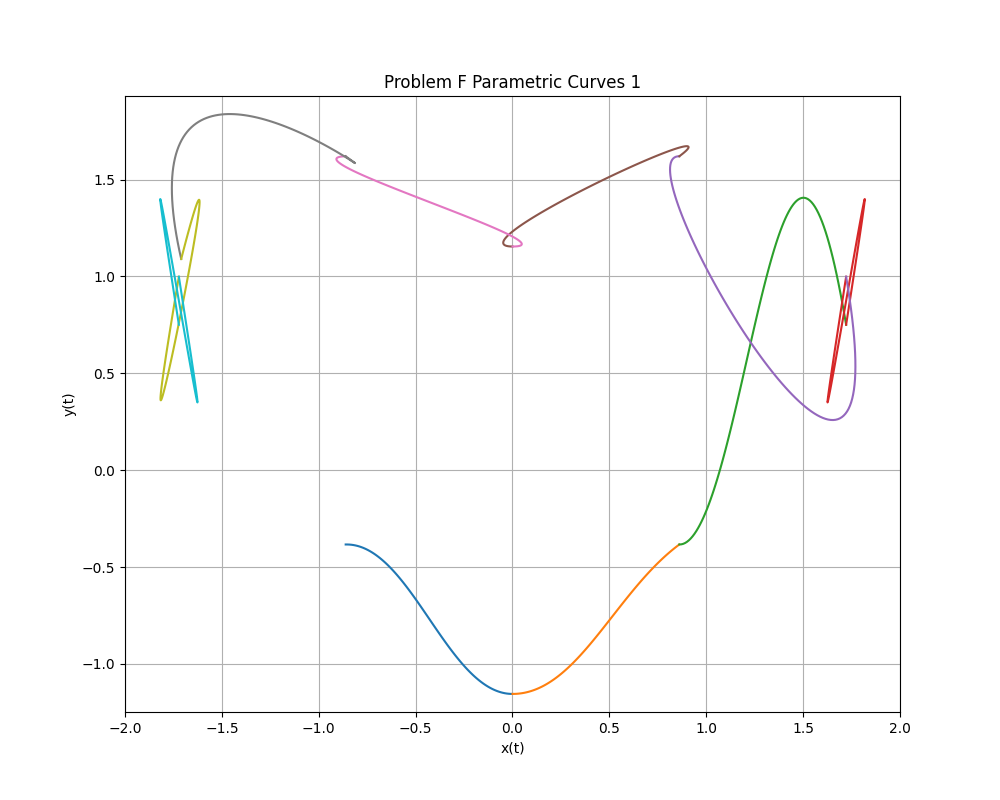
\includegraphics[width=\textwidth]{Pictures/ProblemF_1.png}
        \label{fig:ProblemF1}
    \end{subfigure}
    \hfill
    \begin{subfigure}[b]{0.45\textwidth}
        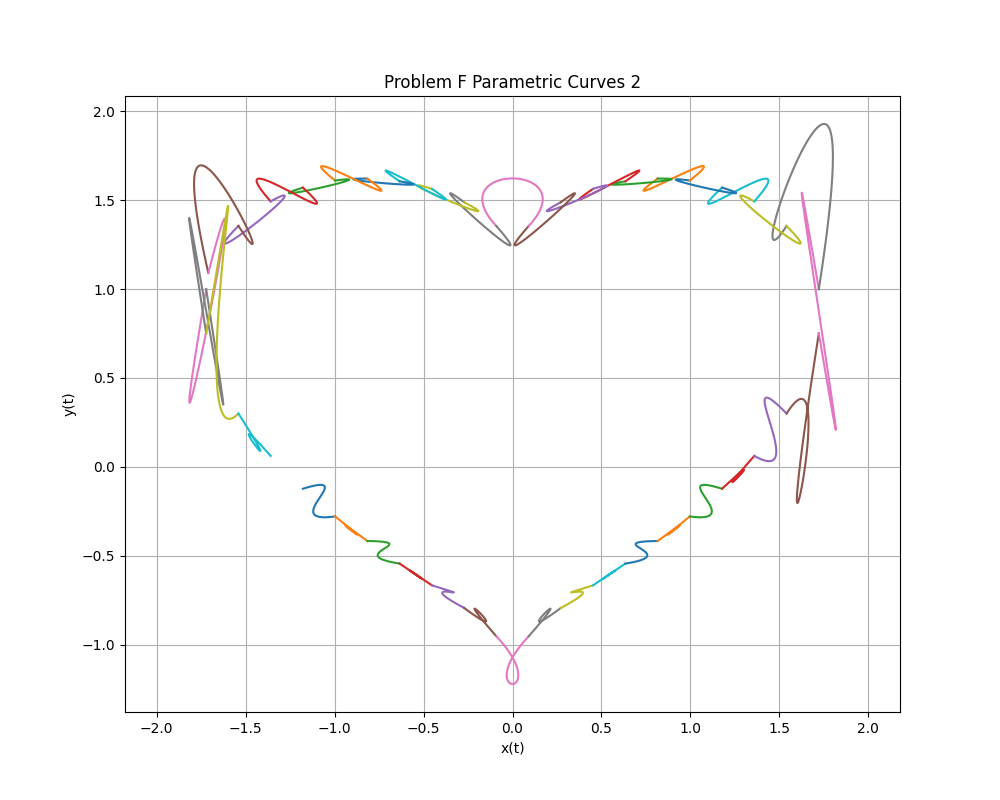
\includegraphics[width=\textwidth]{Pictures/ProblemF_2.png}
        \label{fig:ProblemF2}
    \end{subfigure}

\end{figure}

\begin{figure}[h]
    \centering
    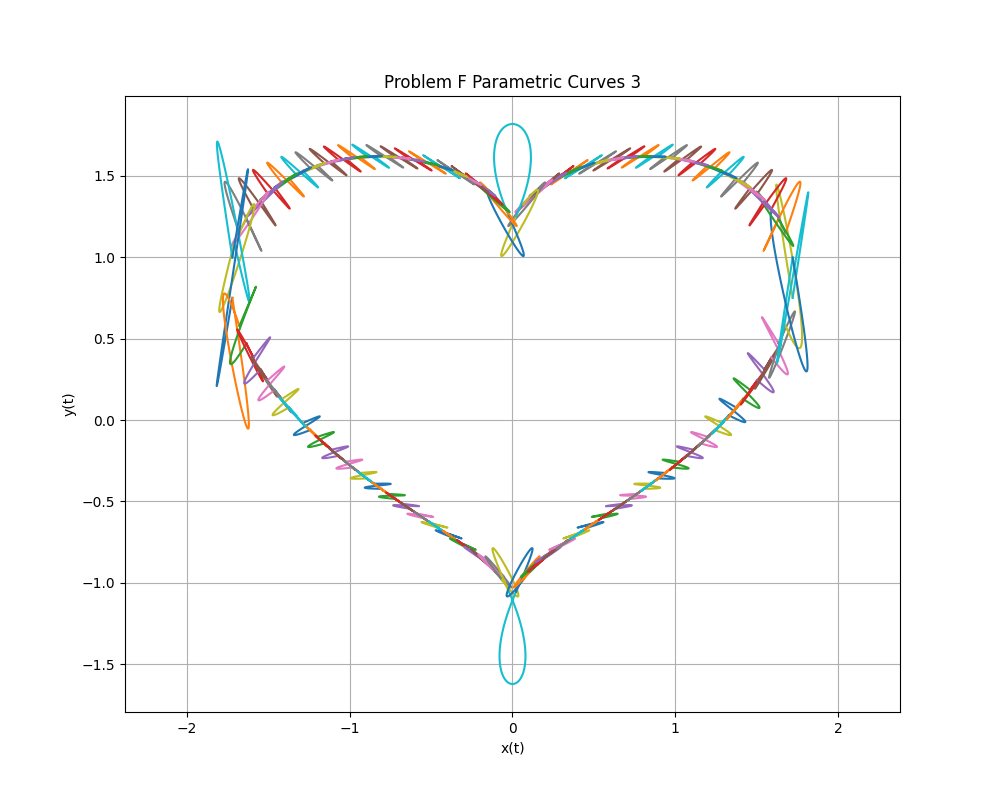
\includegraphics[width=0.5\linewidth]{Pictures/ProblemF_3.png}
    \label{fig:enter-label}
\end{figure}

It can be seen that as \( m \) increases, the Bezier curve gradually gets closer to the heart-shaped curve.

However, there are still some problems, such as at \( x=0 \) and at \( x = -\sqrt3 \) and \( x = \sqrt3 \), due to non-differentiability, the fitting effect is poor, so the appropriate selection of the find\_points interval is very important.

% =======================
\section*{References}
\begin{itemize}
   \item handoutsNumPDEs
   \item ChatGPT, \textit{AI Language Model}, OpenAI Platform, 2024.
\end{itemize}

\end{document}

